\documentclass{article}

\usepackage[utf8]{inputenc}
\usepackage{graphicx}    % Required for inserting images
\usepackage{float}       % To control figure placement
\usepackage{caption}     % Custom captions for figures
\usepackage{subcaption}  % Sub-figures and sub-captions
\usepackage{xcolor}      % Required for colors in listings
\usepackage{listings}    % Code listings
\usepackage[colorlinks=true, linkcolor=blue, hidelinks]{hyperref} % Hyperlinks
\usepackage{minted}
\usepackage{geometry}

% Configuración global para minted
\setminted{
    breaklines=true,          % Habilita el ajuste de línea
    breakanywhere=true,       % Permite el corte de línea en cualquier punto
    fontsize=\small,          % Tamaño de fuente pequeño
    frame=single,             % Cuadro alrededor del código
    bgcolor=lightgray,        % Fondo gris claro
    linenos=true,             % Mostrar números de línea
    tabsize=4,                % Tamaño de tabulaciones
}

% Configuración de márgenes
\geometry{
    left=2.5cm, 
    right=2.5cm, 
    top=3cm, 
    bottom=3cm
}

% Configuración para lstlisting (resaltado de sintaxis)
\lstdefinestyle{bashStyle}{
    language=bash,
    backgroundcolor=\color{lightgray}, % Fondo gris claro
    basicstyle=\ttfamily\small,
    frame=single,
    keywordstyle=\color{blue}\bfseries, % Azul para palabras clave
    commentstyle=\color{gray}\itshape,  % Gris para comentarios
    stringstyle=\color{purple},         % Púrpura para cadenas
    showstringspaces=false,
    breaklines=true,
    postbreak=\mbox{\textcolor{gray}{$\hookrightarrow$}\space},
    columns=fullflexible,
    tabsize=4, % Tamaño de tabulaciones
    literate=% Manejo de caracteres especiales en español
        {á}{{\'a}}1 {é}{{\'e}}1 {í}{{\'i}}1 {ó}{{\'o}}1 {ú}{{\'u}}1
        {Á}{{\'A}}1 {É}{{\'E}}1 {Í}{{\'I}}1 {Ó}{{\'O}}1 {Ú}{{\'U}}1
        {ñ}{{\~n}}1 {Ñ}{{\~N}}1
}

\title{Memoria pr1 BBDD 2}
\author{873983 873983}
\date{February 2025}

\begin{document}

\begin{titlepage}
    \begin{center}
        
\includegraphics[width=\textwidth]{logo.png}
        \vspace{2 cm}
        {\bfseries\LARGE Universidad de Zaragoza \par}
        \vspace{0.5 cm}
        {\scshape\Large Facultad de Ingenier\'ia \par}
        \vspace{0.5 cm}
        {\scshape\LARGE Memoria Práctica 1 \par}
        \vspace{0.5 cm}
        {\scshape\LARGE Bases de Datos 2 \par}
        \vspace{2 cm}
        {\scshape\LARGE Miércoles A 9:00-11:00\par}
        \vspace{0.5 cm}
        {\Large Sergio Isla Lasheras - 873983\par}
        \vspace{0.5 cm}
        {\Large Irene Pascual Albericio - 871627\par}
        \vspace{0.5 cm}
        {\Large Athanasios Usero Samarás - 839543\par}
        \vfill
        {\Large Febrero de 2025 \par}
    \end{center}
\end{titlepage}

%%--INDICE--
\tableofcontents
\newpage

%%--INTRODUCCIÓN--
\section{Introduction}
El objetivo de la presente práctica es el de instalar y configurar los diversos sistemas gestores de bases de datos con los que se trabajará posteriormente en las sesiones prácticas de la asignatura. Pero además, se aprovechará la ocasión para introducirse en las particularidades (aunque a grandes rasgos) de cada sistema gestor: como se gestionan los usuarios, roles y credenciales, como se estructura el espacio de trabajo, construcción semántica y sintáctica de las bases de datos y operaciones de consulta y manipulación básicas; así como sistema de puertos y conectividad externa.

\newpage
\subsection{IBM DB2}
A continuación, indicamos los pasos seguidos para cada una de las tareas solicitadas a realizar:
\subsubsection{Creación de un superusuario, con credenciales seguras, y verificación de que podemos conectarnos con dicho usuario.}
Lo primero que hemos realizado ha sido ejecutar una terminal dentro del contenedor con la imagen del SGBD IBM DB2 ejecutando el siguiente comando:
\begin{lstlisting}[style=bashStyle]
# Verifica que el contenedor db2-db está corriendo
docker ps | grep db2
\end{lstlisting}

Una vez hemos verificado que el contenedor está corriendo, lo próximo a realizar es ejecutar una terminal dentro del contenedor, a la cual accedemos por primera vez con el usuario \textit{root}.
\begin{lstlisting}[style=bashStyle]
# Ejecutar una terminal dentro del contenedor
docker exec -it db2 bash
\end{lstlisting}

A continuación, se procede a crear el usuario \textit{admin} cuya contraseña va a ser igual al nombre.
\begin{lstlisting}[style=bashStyle]
# Crear el usuario admin
useradd -m -d /home/admin -s /bin/bash admin
# Configurar contraseña del superusuario
echo "admin:admin" | chpasswd
\end{lstlisting}

Una vez realizados estos pasos, hay que cambiar al usuario que viene definido en el docker (es decir, \textit{db2inst1}) y entrar a la consola del SGBD donde vamos a crear una base de datos, llamada \textit{ibm\_bbdd}, donde se le concederán todos los permisos al usuario creado anteriormente para convertirlo en superusuario.
\begin{lstlisting}[style=bashStyle]
# Cambiar de usuario
su - db2inst1
# Entrar a la consola del SGBD
db2start
# Crear la base de datos ibm_bbdd
db2 create database ibm_bbdd
# Conectar a la base de datos
db2 connect to ibm_bbdd
\end{lstlisting}
Tras crear la base de datos en el SGBD y conectarnos a ella, ahora vamos a crear un rol que va a representar al superusuario dentro de dicha base de datos y le vamos a dar al usuario que hemos creado anteriormente dicho rol.
\begin{lstlisting}[style=bashStyle]
    # Crear rol superusuario
    db2 create role superadmin
    # Conceder permisos a dicho rol para que sea superusuario
    db2 GRANT DBADM,SECADM,DATAACCESS,ACCESSCTRL ON DATABASE TO ROLE superadmin
    # Asociar al usuario ibm\_db2_admin el rol de superadmin
    db2 GRANT ROLE superadmin TO USER admin
    # Conceder permiso al usuario admin para conectarse a la base de datos
    db2 GRANT CONNECT ON DATABASE TO USER admin
\end{lstlisting}
Tras haber realizado todos los comandos descritos anteriormente, ahora al ejecutar el comando \textit{db2 connect to ibm\_bbdd user admin using admin} nos podemos conectar sin problemas a la base de datos que hemos creado.
\subsubsection{Creación de la estructura básica del espacio de datos}
Para este apartado se ha creado una serie de ficheros \textit{.sql} que definen la creación de la base de datos, las inserciones, las consultas SQL y la eliminación de la misma.
\newline
Para la ejecución de dichos ficheros en IBM es necesario introducir el siguiente comando:
\begin{lstlisting}[style=bashStyle]
    # Ejecutar un fichero .sql en IBM 
    # Donde pone fichero, estaría el nombre del fichero que se desea ejecutar
    db2 -tvf /tmp/{fichero}.sql
\end{lstlisting}
\\
En el fichero \textit{create\_database.sql} se ha creado la base de datos \textbf{GESTION} y dentro de esta el schema \textbf{MEDICA}, donde estarán definidas las tablas. A continuación, se muestra el contenido del fichero:
\begin{minted}[fontsize=\small]{text}
-- Crear la Base de Datos
CREATE DATABASE GESTION;
CONNECT TO GESTION;

-- Crear el Esquema
CREATE SCHEMA MEDICA;
SET CURRENT SCHEMA MEDICA;

-- Crear tabla de médicos
CREATE TABLE MEDICA.MEDICOS (
    dni VARCHAR(9) NOT NULL PRIMARY KEY,
    numLicencia INTEGER NOT NULL UNIQUE,
    nombre VARCHAR(100) NOT NULL,
    especialidad VARCHAR(100) NOT NULL,
    telefono VARCHAR(15)
);

-- Crear tabla de pacientes
CREATE TABLE MEDICA.PACIENTES (
    dni VARCHAR(9) NOT NULL PRIMARY KEY,
    nss INTEGER NOT NULL UNIQUE,
    nombre VARCHAR(100),
    telefono VARCHAR(15)
);

-- Crear tabla de pruebas médicas
CREATE TABLE MEDICA.PRUEBAS (
    id INTEGER GENERATED ALWAYS AS IDENTITY PRIMARY KEY,
    dni_medico VARCHAR(9) NOT NULL,
    dni_paciente VARCHAR(9) NOT NULL,
    tipo_prueba VARCHAR(100),
    fecha DATE,
    resultado VARCHAR(200),
    FOREIGN KEY (dni_medico) REFERENCES MEDICA.MEDICOS(dni),
    FOREIGN KEY (dni_paciente) REFERENCES MEDICA.PACIENTES(dni)
);

-- Verificar las tablas creadas
LIST TABLES FOR SCHEMA MEDICA;

-- Confirmar la estructura de las tablas
DESCRIBE TABLE MEDICA.MEDICOS;
DESCRIBE TABLE MEDICA.PACIENTES;
DESCRIBE TABLE MEDICA.PRUEBAS;

-- Desconectar de la base de datos
CONNECT RESET;

\end{minted}
\newline
Para confirmar que se ha generado correctamente las tablas, el esquema y la base de datos se han realizado los siguientes comandos:
\begin{lstlisting}[style=bashStyle]
    # Conectar a la base de datos creada por el script
    db2 CONNECT TO GESTION
    # Listar las tablas creadas dentro del esquema de la base de datos
    db2 LIST TABLES FOR SCHEMA MEDICA
\end{lstlisting}
Tras ejecutar el último comando, hemos podido visualizar la correcta creación de las tres tablas.

Para la inserción de datos se ha empleado el siguiente fichero \textit{insert\_data.sql}
\begin{minted}[fontsize=\small]{text}
-- Conectar a la base de datos
CONNECT TO GESTION;

-- Insertar en la tabla MEDICOS evitando duplicados
MERGE INTO MEDICA.MEDICOS AS T
USING (VALUES ('12345678A', 98765, 'Dr. Juan Pérez', 'Cardiología', 600123456)) AS S(DNI, NUMLICENCIA, NOMBRE, ESPECIALIDAD, TELEFONO)
ON T.DNI = S.DNI AND T.NUMLICENCIA = S.NUMLICENCIA
WHEN NOT MATCHED THEN
    INSERT (DNI, NUMLICENCIA, NOMBRE, ESPECIALIDAD, TELEFONO)
    VALUES (S.DNI, S.NUMLICENCIA, S.NOMBRE, S.ESPECIALIDAD, S.TELEFONO);

MERGE INTO MEDICA.MEDICOS AS T
USING (VALUES ('87654321B', 12366, 'Dr. Ana Gómez', 'Neurología', 611987654)) AS S(DNI, NUMLICENCIA, NOMBRE, ESPECIALIDAD, TELEFONO)
ON T.DNI = S.DNI AND T.NUMLICENCIA = S.NUMLICENCIA
WHEN NOT MATCHED THEN
    INSERT (DNI, NUMLICENCIA, NOMBRE, ESPECIALIDAD, TELEFONO)
    VALUES (S.DNI, S.NUMLICENCIA, S.NOMBRE, S.ESPECIALIDAD, S.TELEFONO);

-- Insertar en la tabla PACIENTES evitando duplicados
MERGE INTO MEDICA.PACIENTES AS T
USING (VALUES ('11111111A', 1000001, 'Carlos López', 654123988)) AS S(DNI, NSS, NOMBRE, TELEFONO)
ON T.DNI = S.DNI AND T.NSS = S.NSS
WHEN NOT MATCHED THEN
    INSERT (DNI, NSS, NOMBRE, TELEFONO)
    VALUES (S.DNI, S.NSS, S.NOMBRE, S.TELEFONO);

MERGE INTO MEDICA.PACIENTES AS T
USING (VALUES ('22222222B', 1000002, 'María Fernández', 623987654)) AS S(DNI, NSS, NOMBRE, TELEFONO)
ON T.DNI = S.DNI AND T.NSS = S.NSS
WHEN NOT MATCHED THEN
    INSERT (DNI, NSS, NOMBRE, TELEFONO)
    VALUES (S.DNI, S.NSS, S.NOMBRE, S.TELEFONO);

MERGE INTO MEDICA.PACIENTES AS T
USING (VALUES ('33333333C', 1000003, 'Pedro Sánchez', 698741236)) AS S(DNI, NSS, NOMBRE, TELEFONO)
ON T.DNI = S.DNI AND T.NSS = S.NSS
WHEN NOT MATCHED THEN
    INSERT (DNI, NSS, NOMBRE, TELEFONO)
    VALUES (S.DNI, S.NSS, S.NOMBRE, S.TELEFONO);

MERGE INTO MEDICA.PACIENTES AS T
USING (VALUES ('44444444D', 1000004, 'Lucía Rodríguez', 677852963)) AS S(DNI, NSS, NOMBRE, TELEFONO)
ON T.DNI = S.DNI AND T.NSS = S.NSS
WHEN NOT MATCHED THEN
    INSERT (DNI, NSS, NOMBRE, TELEFONO)
    VALUES (S.DNI, S.NSS, S.NOMBRE, S.TELEFONO);

-- Insertar en la tabla PRUEBAS evitando duplicados
MERGE INTO MEDICA.PRUEBAS AS T
USING (VALUES ('11111111A', '12345678A', 'Electrocardiograma', DATE('2024-02-15'), 'Normal')) AS S(DNI_PACIENTE, DNI_MEDICO, TIPO_PRUEBA, FECHA, RESULTADO)
ON T.DNI_PACIENTE = S.DNI_PACIENTE AND T.DNI_MEDICO = S.DNI_MEDICO
WHEN NOT MATCHED THEN
    INSERT (DNI_PACIENTE, DNI_MEDICO, TIPO_PRUEBA, FECHA, RESULTADO)
    VALUES (S.DNI_PACIENTE, S.DNI_MEDICO, S.TIPO_PRUEBA, S.FECHA, S.RESULTADO);

MERGE INTO MEDICA.PRUEBAS AS T
USING (VALUES ('22222222B', '12345678A', 'Ecografía', DATE('2024-02-10'), 'Sin anomalías')) AS S(DNI_PACIENTE, DNI_MEDICO, TIPO_PRUEBA, FECHA, RESULTADO)
ON T.DNI_PACIENTE = S.DNI_PACIENTE AND T.DNI_MEDICO = S.DNI_MEDICO
WHEN NOT MATCHED THEN
    INSERT (DNI_PACIENTE, DNI_MEDICO, TIPO_PRUEBA, FECHA, RESULTADO)
    VALUES (S.DNI_PACIENTE, S.DNI_MEDICO, S.TIPO_PRUEBA, S.FECHA, S.RESULTADO);

MERGE INTO MEDICA.PRUEBAS AS T
USING (VALUES ('33333333C', '87654321B', 'Resonancia magnética', DATE('2024-02-18'), 'Lesión detectada en L3-L4')) AS S(DNI_PACIENTE, DNI_MEDICO, TIPO_PRUEBA, FECHA, RESULTADO)
ON T.DNI_PACIENTE = S.DNI_PACIENTE AND T.DNI_MEDICO = S.DNI_MEDICO
WHEN NOT MATCHED THEN
    INSERT (DNI_PACIENTE, DNI_MEDICO, TIPO_PRUEBA, FECHA, RESULTADO)
    VALUES (S.DNI_PACIENTE, S.DNI_MEDICO, S.TIPO_PRUEBA, S.FECHA, S.RESULTADO);

MERGE INTO MEDICA.PRUEBAS AS T
USING (VALUES ('44444444D', '87654321B', 'Análisis de sangre', DATE('2024-02-15'), 'Niveles normales')) AS S(DNI_PACIENTE, DNI_MEDICO, TIPO_PRUEBA, FECHA, RESULTADO)
ON T.DNI_PACIENTE = S.DNI_PACIENTE AND T.DNI_MEDICO = S.DNI_MEDICO
WHEN NOT MATCHED THEN
    INSERT (DNI_PACIENTE, DNI_MEDICO, TIPO_PRUEBA, FECHA, RESULTADO)
    VALUES (S.DNI_PACIENTE, S.DNI_MEDICO, S.TIPO_PRUEBA, S.FECHA, S.RESULTADO);

-- Desconectar de la base de datos
CONNECT RESET;
\end{minted}

Para probar las consultas en este gestor, se han hecho consultas simples sobre listar los datos de cada una de las tablas de la base de datos que se describen en el fichero \textit{querys.sql}:
\begin{minted}[fontsize=\small]{text}
    -- Conectar a la base de datos GESTION
    CONNECT TO GESTION;
    
    -- Consultar y listar médicos si hay registros
    SELECT * FROM MEDICA.MEDICOS
    WHERE (SELECT COUNT(*) FROM MEDICA.MEDICOS) > 0;
    
    -- Consultar y listar pacientes si hay registros
    SELECT * FROM MEDICA.PACIENTES
    WHERE (SELECT COUNT(*) FROM MEDICA.PACIENTES) > 0;
    
    -- Consultar y listar pruebas si hay registros
    SELECT * FROM MEDICA.PRUEBAS
    WHERE (SELECT COUNT(*) FROM MEDICA.PRUEBAS) > 0;
    
    -- Desconectar de la base de datos
    CONNECT RESET;    
\end{minted}

Para eliminar todos los datos, tablas, esquema y base de datos se ha empleado el fichero \textit{delete\_database.sql}:
\begin{minted}[fontsize=\small]{text}
    -- Conectar a la base de datos GESTION
    CONNECT TO GESTION;
    
    -- Eliminar tablas si existen
    DROP TABLE MEDICA.MEDICOS IF EXISTS;
    DROP TABLE MEDICA.PACIENTES IF EXISTS;
    DROP TABLE MEDICA.PRUEBAS IF EXISTS;
    
    -- Eliminar el esquema si existe
    DROP SCHEMA MEDICA RESTRICT;
    
    -- Desconectarse de la base de datos
    CONNECT RESET;
    
    -- Eliminar la base de datos GESTION
    drop database GESTION;
\end{minted}

\subsubsection{Creación	de usuarios y roles con	distinto acceso	sobre los elementos	del espacio	de datos}
Además del rol superusuario que se ha creado en el primer apartado, se han añadido dos roles más: uno que permite consultar, insertar y actualizar (que hemos llamado writer) y otro que solo permite consultar (que hemos llamado reader).
Lo primero de todo ha sido añadir dos usuarios al sistema:
\begin{lstlisting}[style=bashStyle]
    # Crear el usuario writer
    useradd -m -d /home/writer -s /bin/bash writer
    # Crear el usuario reader
    useradd -m -d /home/reader -s /bin/bash reader
    # Configurar contraseña del usuario writer
    echo "writer:writer" | chpasswd
    # Configurar contraseña del usuario reader
    echo "reader:reader" | chpasswd
\end{lstlisting}
Una vez creados, hay que acceder nuevamente a la terminal del contenedor y configurar los roles.
\begin{lstlisting}[style=bashStyle]
    docker exec -it contenedor_db2 bash
    su - db2inst1
    db2 CONNECT TO GESTION
    # Crear y configurar rol writerrole
    db2 CREATE ROLE writerrole
    db2 GRANT CONNECT ON DATABASE TO writerrole
    db2 GRANT SELECT, INSERT, UPDATE ON MEDICA.MEDICOS TO writerrole
    db2 GRANT SELECT, INSERT, UPDATE ON MEDICA.PACIENTES TO writerrole
    db2 GRANT SELECT, INSERT, UPDATE ON MEDICA.PRUEBAS TO writerrole
    # Crear y configurar rol readerrole
    db2 CREATE ROLE readerrole
    db2 GRANT CONNECT ON DATABASE TO readerrole
    db2 GRANT SELECT ON MEDICA.MEDICOS TO readerrole
    db2 GRANT SELECT ON MEDICA.PACIENTES TO readerrole
    db2 GRANT SELECT ON MEDICA.PRUEBAS TO readerrole
    # Asignar los roles a los respectivos usuarios creados
    db2 GRANT CONNECT ON DATABASE TO USER writer
    db2 GRANT ROLE writerrole TO writer
    db2 GRANT CONNECT ON DATABASE TO USER reader
    db2 GRANT ROLE readerrole TO reader
\end{lstlisting}

\subsection{Oracle}
Instalar Oracle Database en Docker facilita la gestión de bases de datos ofreciendo un entorno consistente y aislado. Este método utiliza Docker para correr Oracle en un contenedor, permitiendo una configuración y despliegue rápidos. Antes de la instalación, se requiere descargar Oracle Instant Client y SQL*Plus, ajustar las variables de entorno y obtener la imagen adecuada de Docker. Este proceso simplifica la operación de Oracle, haciendo su manejo más accesible y eficiente para usuarios de todos los niveles.
\subsubsection{Preparación del Entorno Oracle en Docker}
Asegúrate de que el contenedor de Oracle está operativo y listo para la conexión.

\begin{lstlisting}[style=bashStyle]
docker ps | grep oracle-xe
\end{lstlisting}
Si el contenedor no está corriendo, inícialo desplegando de nuevo en base al \texttt{docker-compose.yml}.

\subsubsection{Configuración del Cliente Oracle Instant en la Máquina Local}
Instala y configura el cliente Oracle para permitir conexiones locales y manipulación de la base de datos.

\begin{lstlisting}[style=bashStyle]
#Instalar dependencias necesarias
sudo apt update
sudo apt install alien libaio1 wget
\end{lstlisting}

\begin{lstlisting}[style=bashStyle]
#Descargar Oracle Instant Client
wget https://download.oracle.com/otn_software/linux/instantclient/2370000/instantclient-basic-linux.x64-23.7.0.25.01.zip
\end{lstlisting}

\begin{lstlisting}[style=bashStyle]
#Crear directorio y descomprimir el archivo
mkdir -p ~/instantclient_23_7
unzip instantclient-basic-linux.x64-23.7.0.25.01.zip -d ~/instantclient_23_7
\end{lstlisting}

\subsubsection{Configurar las variables de entorno}

Edita el archivo \texttt{.bashrc} y añade las siguientes líneas:

\begin{lstlisting}[style=bashStyle]
export ORACLE_HOME=$HOME/instantclient_23_7/instantclient_23_7
export LD_LIBRARY_PATH=$ORACLE_HOME
export PATH=$PATH:$ORACLE_HOME
source ~/.bashrc
\end{lstlisting}

\subsubsection{Descargar y Configurar SQL*Plus}
Instala SQL*Plus para ejecutar comandos SQL desde la línea de comandos.

\begin{lstlisting}[style=bashStyle]
#Descargar SQL*Plus
wget https://download.oracle.com/otn_software/linux/instantclient/2370000/instantclient-sqlplus-linux.x64-23.7.0.25.01.zip
\end{lstlisting}

\begin{lstlisting}[style=bashStyle]
#Descomprimir SQL*Plus
unzip instantclient-sqlplus-linux.x64-23.7.0.25.01.zip -d ~/instantclient_23_7
\end{lstlisting}

\subsubsection{Conectar a Oracle Usando SQL*Plus}
En Oracle Database, el usuario \texttt{sys} es uno de los usuarios más importantes y tiene privilegios de superusuario. Se le considera el usuario administrador principal y es utilizado para realizar tareas de administración de alto nivel. 

Establece una conexión inicial con la base de datos.

\subsubsection{}
\begin{lstlisting}
docker exec -it oracle-xe bash
\end{lstlisting}

\subsubsection{La contraseña/password, debe ser la misma que hemos introducido en el \texttt{docker-file.yml}.}
\begin{lstlisting}[style=bashStyle]
sqlplus sys/password@//localhost:1521/XE as sysdba
\end{lstlisting}

\subsubsection{Operaciones Básicas en Oracle}
Configuraciones iniciales, creación de usuarios y tablespaces.
\vspace{5mm}

\subsubsection{Creación de superusuarios:}

En Oracle, el término "usuario común" no implica que tenga privilegios limitados o normales. Se refiere específicamente a que el usuario puede acceder y operar en todas las bases de datos pluggables (PDBs) dentro de una base de datos contenedora (CDB) en una configuración multitenant. 

Cuando un "usuario común" como superadmin recibe el rol de DBA, se convierte en un superusuario debido a los privilegios administrativos extensos que este rol le permite, como: control total sobre aspectos críticos y administrativos de la base de datos, gestionar usuarios, configurar la seguridad, manejar copias de seguridad, etc.
\begin{lstlisting}[style=bashStyle]
#Creación del superusuario
CREATE USER c##superadmin IDENTIFIED BY Admin1234;
GRANT DBA TO c##superadmin;
\end{lstlisting}

\vspace{5mm}

\subsubsection{Creación de tablespaces}

Un tablespace en Oracle es un contenedor de almacenamiento que guarda los datos. Es esencial configurar tablespaces antes de crear usuarios, ya que determinan dónde se almacenarán los datos de estos.

Antes de crear un tablespace, es muy importante seleccionar el contenedor adecuado para asegurarse de que los datos se almacenen en la ubicación correcta, especialmente en configuraciones multitenant. 

El proceso comienza con la verificación de las PDBs disponibles:

\begin{lstlisting}[style=bashStyle]
-- Mostrar todas las PDBs disponibles en la instancia de Oracle
SHOW PDBS;

CON_ID CON_NAME                       OPEN MODE  RESTRICTED
------- ------------------------------ ---------- ----------
    2 PDB$SEED                       READ ONLY  NO
    3 XEPDB1                         READ WRITE NO
\end{lstlisting}

Una vez identificada la PDB deseada, cambiamos la sesión a esa PDB específica:

\begin{lstlisting}[style=bashStyle]
-- Cambiar la sesión al contenedor XEPDB1
ALTER SESSION SET CONTAINER=XEPDB1;
\end{lstlisting}

A continuación, se muestra cómo crear un tablespace denominado \texttt{myworkspace1}:

\begin{lstlisting}[style=bashStyle]
CREATE TABLESPACE myworkspace DATAFILE 'myworkspace1.dbf' SIZE 100M AUTOEXTEND ON NEXT 10M MAXSIZE UNLIMITED;
\end{lstlisting}

\vspace{5mm}
\subsubsection{Creación de usuarios de escritura y lectura:}

Primero, creamos el usuario \texttt{writer}. Este proceso se realiza mediante un comando SQL que especifica una contraseña para el usuario y el tablespace predeterminado donde se almacenarán los objetos que \texttt{writer} cree. 

El comando es el siguiente:

\begin{lstlisting}[style=bashStyle]
CREATE USER writer IDENTIFIED BY writerPass DEFAULT TABLESPACE myworkspace1;
\end{lstlisting}

Este paso es crucial porque establece las credenciales de \texttt{writer} y define dónde se guardarán físicamente los datos que el usuario maneje, facilitando una organización lógica y eficiente del espacio en la base de datos.

Al crear el usuario \texttt{writer}, también necesitamos asignarle privilegios básicos que le permitirán operar dentro de la base de datos: realizar funciones básicas necesarias, modificar cualquier tabla, crear secuencias para autoincrementos, definir vistas y crear sinónimos.

\begin{lstlisting}[style=bashStyle]
-- Privilegios inciales:
GRANT CREATE SESSION, CREATE TABLE TO writer;

-- Privilegios adicionales:
GRANT ALTER ANY TABLE, CREATE SEQUENCE, CREATE VIEW, CREATE SYNONYM TO writer;
\end{lstlisting}

Luego, procedemos a crear el usuario \texttt{reader}, similar a \texttt{writer}, pero con privilegios más limitados adecuados para un perfil que solo requiere leer datos:

\begin{lstlisting}[style=bashStyle]
CREATE USER reader IDENTIFIED BY readerPass DEFAULT TABLESPACE myworkspace1;
\end{lstlisting}

Para \texttt{reader}, solo otorgamos el privilegio de CREATE SESSION, que es suficiente para que acceda a la base de datos sin permitirle ni modificarla ni crear nuevos objetos:

\begin{lstlisting}[style=bashStyle]
GRANT CREATE SESSION TO reader;
\end{lstlisting}

Cuando se termine el siguiente apartado de "Creación de tablas" que hay a continuación, se deben ejecutar estos comandos, para poder otorgar correctamente los privilegios de lectura al usuario lector de las tablas creadas:

\begin{lstlisting}[style=bashStyle]
-- Conexión como SYSDBA
CONNECT sys/oracle123@//localhost:1521/XEPDB1 AS SYSDBA;

-- Otorgamos privilegios
GRANT SELECT ON WRITER.medicos TO reader;
GRANT SELECT ON WRITER.pacientes TO reader;
GRANT SELECT ON WRITER.pruebas TO reader;
\end{lstlisting}

\subsubsection{Creación e inserción de tablas}
Para la creación de tablas, se ejecuta un archivo de script SQL denominado "CreacionTablasOracle", que contiene todos los comandos necesarios para definir las tablas y las relaciones entre ellas de médicos, pacientes y pruebas. 

El contenido del script "CreacionTablasOracle.sql" incluye:

\begin{lstlisting}[style=bashStyle]
    -- Conectar al usuario writer con su contraseña
    CONNECT writer/writerPass@localhost:1521/XEPDB1;
    SHOW USER;
    
    -- Eliminar las tablas si ya existen, y si no, no se hace nada
    BEGIN
        EXECUTE IMMEDIATE 'DROP TABLE pruebas CASCADE CONSTRAINTS';
    EXCEPTION
        WHEN OTHERS THEN
            NULL;  
    END;
    /
    
    BEGIN
        EXECUTE IMMEDIATE 'DROP TABLE pacientes CASCADE CONSTRAINTS';
    EXCEPTION
        WHEN OTHERS THEN
            NULL; 
    END;
    /
    
    BEGIN
        EXECUTE IMMEDIATE 'DROP TABLE medicos CASCADE CONSTRAINTS';
    EXCEPTION
        WHEN OTHERS THEN
            NULL;  
    END;
    /
    
    -- Crear la tabla de médicos
    CREATE TABLE medicos (
        dni VARCHAR2(9) PRIMARY KEY,
        numLicencia NUMBER NOT NULL UNIQUE,
        nombre VARCHAR2(100) NOT NULL,
        especialidad VARCHAR2(100) NOT NULL,
        telefono VARCHAR2(15)
    );
    
    -- Crear la tabla de pacientes
    CREATE TABLE pacientes (
        dni VARCHAR2(9) PRIMARY KEY,
        nss NUMBER NOT NULL UNIQUE,
        nombre VARCHAR2(100),
        telefono VARCHAR2(15)
    );
    
    -- Crear la tabla de pruebas médicas
    CREATE TABLE pruebas (
        id NUMBER GENERATED ALWAYS AS IDENTITY PRIMARY KEY,
        dni_medico VARCHAR2(9) NOT NULL,
        dni_paciente VARCHAR2(9) NOT NULL,
        tipo_prueba VARCHAR2(100),
        fecha DATE,
        resultado VARCHAR2(200),
        CONSTRAINT fk_medico FOREIGN KEY (dni_medico) REFERENCES medicos(dni),
        CONSTRAINT fk_paciente FOREIGN KEY (dni_paciente) REFERENCES pacientes(dni)
    );
\end{lstlisting}

Para ejecutar este script utilizando SQL*Plus, se introduce el siguiente comando:

\begin{lstlisting}[style=bashStyle]
nano CreacionTablasOracle.sql
docker cp ~/bd2/oracle/CreacionTablasOracle.sql oracle-xe:/opt/oracle
docker exec -it oracle-xe bash
sqlplus writer/writerPass@localhost:1521/XEPDB1
@/opt/oracle/CreacionTablasOracle.sql
\end{lstlisting}

Tras crear las tablas, hay que conectarse al sistema como el usuario \texttt{sys} utilizando privilegios de SYSDBA. Este nivel de acceso es esencial para realizar ajustes administrativos de alto nivel que afectan la estructura y los límites de almacenamiento de la base de datos.

\begin{lstlisting}[style=bashStyle]
CONNECT sys/oracle123@//localhost:1521/XEPDB1 AS SYSDBA;
\end{lstlisting}

Una vez establecida la conexión, se altera la cuota de almacenamiento del usuario \texttt{writer} para asignarle una cuota ilimitada en el tablespace myworkspace1. Esto asegura que writer tenga suficiente espacio para almacenar datos y crear objetos sin enfrentar restricciones de espacio.

\begin{lstlisting}[style=bashStyle]
ALTER USER writer QUOTA UNLIMITED ON myworkspace1;
\end{lstlisting}

Posteriormente, hay que conectarse de nuevo como \texttt{writer} para realizar operaciones de inserción de datos en las tablas. Este paso lo llevamos a cabo mediante un script denominado "InsercionTablasOracle". 

El contenido del script "InsercionTablasOracle.sql" incluye:

\begin{lstlisting}[style=bashStyle]
    -- Conexión como usuario writer y con su contraseña
    CONNECT writer/writerPass@localhost:1521/XEPDB1;
    
    SET SERVEROUTPUT ON;
    
    -- Comprobación de existencia de la tabla 'medicos' antes de insertar
    BEGIN
        -- Intentar acceder a la tabla 'medicos' en el esquema 'WRITER' con EXECUTE IMMEDIATE
        BEGIN
            EXECUTE IMMEDIATE 'SELECT COUNT(*) FROM WRITER.medicos';
            DBMS_OUTPUT.PUT_LINE('La tabla MEDICOS existe en el esquema WRITER.');
    
            -- Insertar en la tabla 'medicos'
            EXECUTE IMMEDIATE 'INSERT INTO WRITER.medicos (dni, numLicencia, nombre, especialidad, telefono)
                               SELECT ''12345678A'', 98765, ''Dr. Juan Pérez'', ''Cardiología'', ''600123456''
                               FROM dual
                               WHERE NOT EXISTS (SELECT 1 FROM WRITER.medicos WHERE dni = ''12345678A'')';
    
            EXECUTE IMMEDIATE 'INSERT INTO WRITER.medicos (dni, numLicencia, nombre, especialidad, telefono)
                               SELECT ''87654321B'', 12366, ''Dra. Ana Gómez'', ''Neurología'', ''611987654''
                               FROM dual
                               WHERE NOT EXISTS (SELECT 1 FROM WRITER.medicos WHERE dni = ''87654321B'')';
        EXCEPTION
            WHEN OTHERS THEN
                DBMS_OUTPUT.PUT_LINE('La tabla MEDICOS no existe en el esquema WRITER. No se realizarán inserciones.');
        END;
    END;
    /
    
    -- Comprobación de existencia de la tabla 'pacientes' antes de insertar
    BEGIN
        -- Intentar acceder a la tabla 'pacientes' en el esquema 'WRITER' con EXECUTE IMMEDIATE
        BEGIN
            EXECUTE IMMEDIATE 'SELECT COUNT(*) FROM WRITER.pacientes';
            DBMS_OUTPUT.PUT_LINE('La tabla PACIENTES existe en el esquema WRITER.');
    
            -- Insertar en la tabla 'pacientes'
            EXECUTE IMMEDIATE 'INSERT INTO WRITER.pacientes (dni, nss, nombre, telefono)
                               SELECT ''11111111A'', 1000001, ''Carlos López'', ''654123987''
                               FROM dual
                               WHERE NOT EXISTS (SELECT 1 FROM WRITER.pacientes WHERE dni = ''11111111A'')';
    
            EXECUTE IMMEDIATE 'INSERT INTO WRITER.pacientes (dni, nss, nombre, telefono)
                               SELECT ''22222222B'', 1000002, ''María Fernández'', ''623987654''
                               FROM dual
                               WHERE NOT EXISTS (SELECT 1 FROM WRITER.pacientes WHERE dni = ''22222222B'')';
    
            EXECUTE IMMEDIATE 'INSERT INTO WRITER.pacientes (dni, nss, nombre, telefono)
                               SELECT ''33333333C'', 1000003, ''Pedro Sánchez'', ''698741236''
                               FROM dual
                               WHERE NOT EXISTS (SELECT 1 FROM WRITER.pacientes WHERE dni = ''33333333C'')';
    
            EXECUTE IMMEDIATE 'INSERT INTO WRITER.pacientes (dni, nss, nombre, telefono)
                               SELECT ''44444444D'', 1000004, ''Lucía Rodríguez'', ''677852963''
                               FROM dual
                               WHERE NOT EXISTS (SELECT 1 FROM WRITER.pacientes WHERE dni = ''44444444D'')';
        EXCEPTION
            WHEN OTHERS THEN
                DBMS_OUTPUT.PUT_LINE('La tabla PACIENTES no existe en el esquema WRITER. No se realizarán inserciones.');
        END;
    END;
    /
    
    -- Comprobación de existencia de la tabla 'pruebas' antes de insertar
    BEGIN
        -- Intentar acceder a la tabla 'pruebas' en el esquema 'WRITER' con EXECUTE IMMEDIATE
        BEGIN
            EXECUTE IMMEDIATE 'SELECT COUNT(*) FROM WRITER.pruebas';
            DBMS_OUTPUT.PUT_LINE('La tabla PRUEBAS existe en el esquema WRITER.');
    
            -- Insertar en la tabla 'pruebas'
            EXECUTE IMMEDIATE 'INSERT INTO WRITER.pruebas (dni_medico, dni_paciente, tipo_prueba, fecha, resultado)
                               SELECT ''12345678A'', ''11111111A'', ''Electrocardiograma'', TO_DATE(''2024-02-15'', ''YYYY-MM-DD''), ''Normal''
                               FROM dual
                               WHERE NOT EXISTS (SELECT 1 FROM WRITER.pruebas WHERE dni_medico = ''12345678A'' AND dni_paciente = ''11111111A'' AND tipo_prueba = ''Electrocardiograma'' AND fecha = TO_DATE(''2024-02-15'', ''YYYY-MM-DD''))';
    
            EXECUTE IMMEDIATE 'INSERT INTO WRITER.pruebas (dni_medico, dni_paciente, tipo_prueba, fecha, resultado)
                               SELECT ''12345678A'', ''22222222B'', ''Ecografía'', TO_DATE(''2024-02-10'', ''YYYY-MM-DD''), ''Sin anomalías''
                               FROM dual
                               WHERE NOT EXISTS (SELECT 1 FROM WRITER.pruebas WHERE dni_medico = ''12345678A'' AND dni_paciente = ''22222222B'' AND tipo_prueba = ''Ecografía'' AND fecha = TO_DATE(''2024-02-10'', ''YYYY-MM-DD''))';
    
            EXECUTE IMMEDIATE 'INSERT INTO WRITER.pruebas (dni_medico, dni_paciente, tipo_prueba, fecha, resultado)
                               SELECT ''87654321B'', ''33333333C'', ''Resonancia magnética'', TO_DATE(''2024-02-18'', ''YYYY-MM-DD''), ''Lesión detectada en L3-L4''
                               FROM dual
                               WHERE NOT EXISTS (SELECT 1 FROM WRITER.pruebas WHERE dni_medico = ''87654321B'' AND dni_paciente = ''33333333C'' AND tipo_prueba = ''Resonancia magnética'' AND fecha = TO_DATE(''2024-02-18'', ''YYYY-MM-DD''))';
    
            EXECUTE IMMEDIATE 'INSERT INTO WRITER.pruebas (dni_medico, dni_paciente, tipo_prueba, fecha, resultado)
                               SELECT ''87654321B'', ''44444444D'', ''Análisis de sangre'', TO_DATE(''2024-02-20'', ''YYYY-MM-DD''), ''Niveles normales''
                               FROM dual
                               WHERE NOT EXISTS (SELECT 1 FROM WRITER.pruebas WHERE dni_medico = ''87654321B'' AND dni_paciente = ''44444444D'' AND tipo_prueba = ''Análisis de sangre'' AND fecha = TO_DATE(''2024-02-20'', ''YYYY-MM-DD''))';
        EXCEPTION
            WHEN OTHERS THEN
                DBMS_OUTPUT.PUT_LINE('La tabla PRUEBAS no existe en el esquema WRITER. No se realizarán inserciones.');
        END;
    END;
    /
\end{lstlisting}

Para ejecutar este script utilizando SQL*Plus, utilizamos el siguiente comando:

\begin{lstlisting}[style=bashStyle]
nano InsercionTablasOracle.sql
docker cp ~/bd2/oracle/InsercionTablasOracle.sql oracle-xe:/opt/oracle
docker exec -it oracle-xe bash
sqlplus writer/writerPass@localhost:1521/XEPDB1
@/opt/oracle/InsercionTablasOracle.sql
\end{lstlisting}

\subsubsection{Consultas}

En el apartado de consultas, el usuario \texttt{reader} lleva a cabo una serie de operaciones para acceder a la información contenida en las tablas medicos, pacientes y pruebas que fueron previamente creadas y pobladas por el usuario \texttt{writer}. 

El proceso inicia con la conexión a la base de datos Oracle usando las credenciales del usuario \texttt{reader}. 

\begin{lstlisting}[style=bashStyle]
CONNECT reader/readerPass@localhost:1521/XEPDB1;
\end{lstlisting}

Para realizar las consultas han sido agrupadas todas ellas en un script llamado "ConsultasOracle".

El contenido del script "ConsultasOracle.sql" incluye:

\begin{lstlisting}[style=bashStyle]
    -- Conexión como usuario reader con su contraseña
    CONNECT reader/readerPass@localhost:1521/XEPDB1;
    
    -- Comprobación de existencia de la tabla 'medicos' antes de mostrar los datos
    DECLARE
        v_exists NUMBER;
    BEGIN
        SELECT COUNT(*) INTO v_exists
        FROM all_tables
        WHERE table_name = 'MEDICOS' AND owner = 'WRITER';
    
        IF v_exists > 0 THEN
            EXECUTE IMMEDIATE 'SELECT * FROM WRITER.medicos';
        END IF;
    END;
    /
    
    -- Comprobación de existencia de la tabla 'pacientes' antes de mostrar los datos
    DECLARE
        v_exists NUMBER;
    BEGIN
        SELECT COUNT(*) INTO v_exists
        FROM all_tables
        WHERE table_name = 'PACIENTES' AND owner = 'WRITER';
    
        IF v_exists > 0 THEN
            EXECUTE IMMEDIATE 'SELECT * FROM WRITER.pacientes';
        END IF;
    END;
    /
    
    -- Comprobación de existencia de la tabla 'pruebas' antes de mostrar los datos
    DECLARE
        v_exists NUMBER;
    BEGIN
        SELECT COUNT(*) INTO v_exists
        FROM all_tables
        WHERE table_name = 'PRUEBAS' AND owner = 'WRITER';
    
        IF v_exists > 0 THEN
            EXECUTE IMMEDIATE 'SELECT * FROM WRITER.pruebas';
        END IF;
    END;
    /
    
    -- Comprobación de existencia de la tabla 'pacientes' antes de realizar la búsqueda
    DECLARE
        v_exists NUMBER;
    BEGIN
        SELECT COUNT(*) INTO v_exists
        FROM all_tables
        WHERE table_name = 'PACIENTES' AND owner = 'WRITER';
    
        IF v_exists > 0 THEN
            EXECUTE IMMEDIATE 'SELECT * FROM WRITER.pacientes WHERE nombre LIKE ''%María%''';
        END IF;
    END;
    /
    
    -- Comprobación de existencia de la tabla 'pruebas' antes de realizar la consulta por fecha
    DECLARE
        v_exists NUMBER;
    BEGIN
        SELECT COUNT(*) INTO v_exists
        FROM all_tables
        WHERE table_name = 'PRUEBAS' AND owner = 'WRITER';
    
        IF v_exists > 0 THEN
            EXECUTE IMMEDIATE 'SELECT * FROM WRITER.pruebas WHERE fecha = TO_DATE(''2024-02-15'', ''YYYY-MM-DD'')';
        END IF;
    END;
    /
    
    -- Comprobación de existencia de las tablas 'medicos', 'pacientes' y 'pruebas' antes de realizar la consulta detallada
    DECLARE
        v_exists_medicos NUMBER;
        v_exists_pacientes NUMBER;
        v_exists_pruebas NUMBER;
    BEGIN
        SELECT COUNT(*) INTO v_exists_medicos
        FROM all_tables
        WHERE table_name = 'MEDICOS' AND owner = 'WRITER';
    
        SELECT COUNT(*) INTO v_exists_pacientes
        FROM all_tables
        WHERE table_name = 'PACIENTES' AND owner = 'WRITER';
    
        SELECT COUNT(*) INTO v_exists_pruebas
        FROM all_tables
        WHERE table_name = 'PRUEBAS' AND owner = 'WRITER';
    
        IF v_exists_medicos > 0 AND v_exists_pacientes > 0 AND v_exists_pruebas > 0 THEN
            EXECUTE IMMEDIATE '
                SELECT m.nombre AS medico, p.nombre AS paciente, pr.tipo_prueba, pr.fecha, pr.resultado
                FROM WRITER.pruebas pr
                JOIN WRITER.medicos m ON pr.dni_medico = m.dni
                JOIN WRITER.pacientes p ON pr.dni_paciente = p.dni';
        END IF;
    END;
    /
\end{lstlisting}

Para ejecutar este script, se debe ejecutar este comando:
\begin{lstlisting}[style=bashStyle]
sqlplus reader/readerPass@localhost:1521/XEPDB1 @ConsultasOracle.sql
\end{lstlisting}

\subsubsection{Redirección de puertos}

Para gestionar y asegurar la correcta redirección de puertos en la configuración de una base de datos Oracle usando DBeaver Enterprise, se debe descargar e instalar la aplicacion desde el sitio oficial de DBeaver, accesible a través del enlace \textit{\textcolor{blue}{\href{https://dbeaver.com/download/enterprise/}{DBeaver Enterprise}}}. 

Posteriormente, tras el proceso de registro o inicio de sesión en DBeaver, se establece una nueva conexión y se procede a especificar los detalles necesarios para conectar con la base de datos Oracle que se ha creado. 

Estos detalles necesarios, incluyen: el host, usualmente localhost, el puerto estándar 1521 de Oracle, el nombre del servicio de la base de datos, que en este caso fue XEPDB1, etc. 

\begin{figure}[H]
    \centering
    \begin{tabular}{c c}  % Dos columnas centradas
    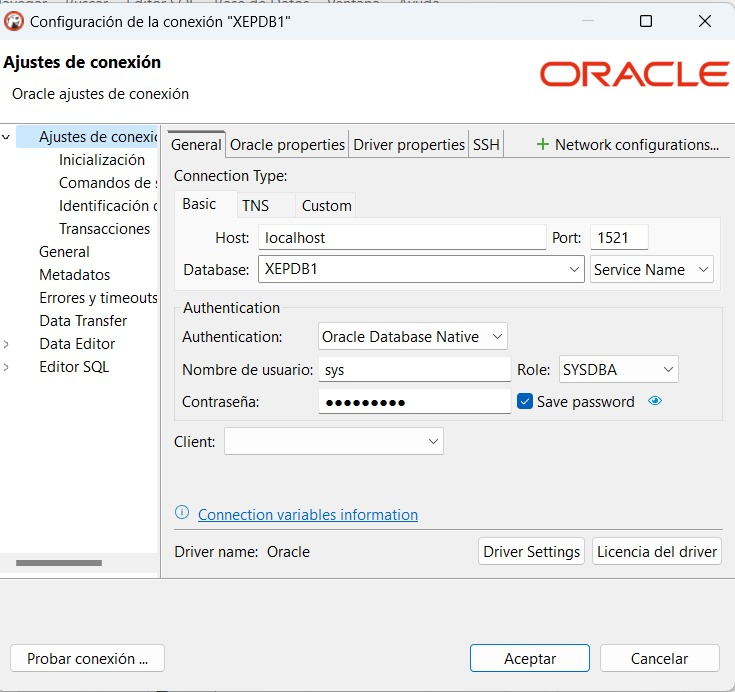
\includegraphics[width=0.6\textwidth]{configuracion_ajustes_conexion_oracle.png}
    \end{tabular}
    \caption{Instalación de la máquina virtual Debian}
    \label{fig:Configuración DBeaver de Oracle}
\end{figure}

Una vez configurados estos parámetros, se realiza una prueba de conexión, desde "Probar conexión...", y si funciona, se pulsa sobre "Aceptar" y se establece la conexión. 

Finalmente, ya tenemos accesible desde DBeaver la base de datos, y se puede modificar, crear, eliminar, consultar... sobre esta base. 


\newpage
\subsection{HBase}
\subsubsection{Introducción}
HBase es un sistema de bases de datos NoSQL escalable basado en HDFS, diseñado para almacenar grandes volúmenes de datos distribuidos. En esta documentación, se describirá el proceso de instalación y configuración de HBase, incluyendo los intentos de integración con Kerberos y la posterior decisión de prescindir de esta tecnología debido a dificultades técnicas.

\subsubsection{Intento de Integración con Kerberos}
Para garantizar una autenticación segura en HBase, se intentó la integración de Kerberos como sistema de gestión de identidades. El objetivo era proporcionar una autenticación basada en tickets para controlar el acceso a los datos. Sin embargo, debido a múltiples problemas técnicos, se decidió desestimar Kerberos y proceder con una configuración sin autenticación centralizada.


\subsubsection{Configuración Inicial de Kerberos}

La instalación de Kerberos en el host se realizó con los siguientes comandos:

\begin{lstlisting}[style=bashStyle]
sudo apt update
sudo apt install -y krb5-kdc krb5-admin-server krb5-user
\end{lstlisting}

A continuación, se configuró el archivo \texttt{/etc/krb5.conf}:

\begin{minted}{text}
[libdefaults]
default_realm = HBASE.LOCAL
dns_lookup_realm = false
dns_lookup_kdc = false
ticket_lifetime = 24h
renew_lifetime = 7d
forwardable = true

[realms]
HBASE.LOCAL = {
    kdc = localhost
    admin_server = localhost
}

[domain_realm]
.hbase.local = HBASE.LOCAL
hbase.local = HBASE.LOCAL
\end{minted}

Se procedió a inicializar la base de datos de Kerberos:

\begin{lstlisting}[style=bashStyle]
sudo krb5_newrealm
\end{lstlisting}

\newpage
Se crearon los principales para HBase Master y RegionServer:

\begin{lstlisting}[style=bashStyle]
sudo kadmin.local -q "addprinc -randkey hbase-master@HBASE.LOCAL"
sudo kadmin.local -q "addprinc -randkey hbase-regionserver@HBASE.LOCAL"
\end{lstlisting}


Y se generaron los keytabs:

\begin{lstlisting}[style=bashStyle]
sudo kadmin.local -q "ktadd -k /etc/hbase/keytabs/hbase-master.keytab hbase-master@HBASE.LOCAL"
sudo kadmin.local -q "ktadd -k /etc/hbase/keytabs/hbase-regionserver.keytab hbase-regionserver@HBASE.LOCAL"
\end{lstlisting}

Estos archivos fueron copiados a los contenedores de HBase:

\begin{lstlisting}[style=bashStyle]
docker cp /etc/hbase/keytabs/hbase-master.keytab hbase-db:/etc/hbase/keytabs/hbase-master.keytab
docker cp /etc/hbase/keytabs/hbase-regionserver.keytab hbase-db:/etc/hbase/keytabs/hbase-regionserver.keytab
\end{lstlisting}

\subsubsection{}
A pesar de la configuración, surgieron diversos problemas que impidieron la correcta autenticación en HBase:

\vspace{5mm}

\subsubsection{Problema con los Keytabs}

Al ejecutar \texttt{klist -kt} dentro del contenedor de HBase, se obtuvo el error:

\begin{lstlisting}[style=bashStyle]
klist: Unsupported key table format version number while starting keytab scan
\end{lstlisting}


Se intentó regenerar los keytabs y copiarlos nuevamente al contenedor sin éxito.

\vspace{5mm}


\subsubsection{Errores en la Autenticación de HBase}

Al ejecutar \texttt{kinit} y listar las regiones en HBase, se obtuvo el error:

\begin{minted}[breaklines=true]{text}
ERROR: No valid credentials provided (Mechanism level: Failed to find any Kerberos tgt)
\end{minted}

Tras varios intentos, se decidió desestimar la configuración de Kerberos.

\subsubsection{Desestimación de Kerberos}
Dado que los problemas con Kerberos dificultaban el desarrollo y consumían demasiado tiempo, se optó por eliminar la configuración de seguridad y proceder sin autenticación:

\vspace{5mm}

\subsubsection{1. Eliminación de Kerberos}

\begin{lstlisting}[style=bashStyle]
docker-compose down
sudo rm -rf /etc/hbase/keytabs
sudo rm -rf /var/lib/krb5kdc
sudo apt-get remove --purge krb5-kdc krb5-admin-server
sudo apt-get autoremove
\end{lstlisting}

\newpage
\subsubsection{2. Modificación de la configuración de HBase}

Se editó el archivo hbase-site.xml para cambiar la autenticación:


\begin{minted}[fontsize=\small]{xml}
hbase.security.authentication
simple

hbase.security.authorization
false
\end{minted}

Luego, se copió el archivo actualizado dentro del contenedor de HBase:

\begin{lstlisting}[style=bashStyle]
docker cp ~/bd2/hbase-config/hbase-site.xml hbase-db:/opt/hbase/conf/hbase-site.xml
\end{lstlisting}


\subsubsection{3. Reinicio de Servicios}

\begin{lstlisting}[style=bashStyle]
docker restart hbase-db
\end{lstlisting}


\subsubsection{4. Verificación de la Configuración}

Para verificar que HBase funcionaba sin Kerberos, se ejecutaron los siguientes comandos:

\begin{lstlisting}[style=bashStyle]
docker exec -it hbase-db hbase shell
\end{lstlisting}

Se intentó crear la tabla `hbase:acl` para la gestión de permisos, pero se observó que **ya existía**, lo que indicaba que la configuración de permisos estaba activa:

\begin{lstlisting}[style=bashStyle]
hbase(main):023:0* create 'hbase:acl', {NAME => 'f', VERSIONS => 1}
ERROR: Table already exists: hbase:acl!
\end{lstlisting}

Para confirmar su existencia, se escaneó su contenido:

\begin{lstlisting}[style=bashStyle]
hbase(main):024:0> scan 'hbase:acl'
ROW                      COLUMN+CELL
0 row(s)
Took 0.0219 seconds
\end{lstlisting}

Finalmente, se verificó el estado del sistema:

\begin{lstlisting}[style=bashStyle]
hbase(main):025:0> status 'detailed'
\end{lstlisting}

Lo importante aquí fue notar la presencia de:

\begin{minted}[fontsize=\small]{text}
master coprocessors: [AccessController]
\end{minted}

Esto confirmó que **el sistema ya tenía habilitados los permisos sin necesidad de Kerberos**.

\subsubsection{Operaciones Básicas en Oracle}

Tras la desestimación de Kerberos, se procedió a la configuración de HBase sin autenticación centralizada. En esta sección se describen las operaciones realizadas para gestionar el acceso de usuarios, la creación de espacios, tablas y la ejecución de consultas.

\subsubsection{Creación superusuarios:}
El primer paso consistió en otorgar permisos administrativos al usuario `admin`. Esto se logró mediante el siguiente comando en HBase Shell:

\begin{lstlisting}[style=bashStyle]
hbase(main):028:0* grant 'admin', 'RWCXA'
Took 0.4414 seconds
\end{lstlisting}

Donde los permisos otorgados fueron:
\begin{minted}[fontsize=\small]{text}
      {R} - Read (Lectura)
      {W} - Write (Escritura)
      {C} - Create (Creación)
      {X} - Execute (Ejecución)
      {A} - Admin (Administración)
\end{minted}

Este comando habilitó al usuario `admin` con privilegios totales sobre la base de datos de HBase.

\subsubsection{Creación de tablespaces}

En HBase, un espacio de nombres (namespace) permite organizar las tablas en una estructura similar a los esquemas en SQL. Se creó un espacio de nombres específico:

\begin{lstlisting}[style=bashStyle]
hbase(main):033:0* create_namespace 'espacioHBase'
Took 0.2981 seconds
\end{lstlisting}

Para verificar la correcta creación del namespace, se ejecutó:

\begin{lstlisting}[style=bashStyle]
hbase(main):034:0> list_namespace
NAMESPACE
espacioHBase
default
hbase
3 row(s)
Took 0.0593 seconds
\end{lstlisting}

El namespace `espacioHBase` apareció correctamente en la lista, junto con los espacios de nombres `default` y `hbase`, confirmando su creación exitosa.


\subsubsection{Creación de usuarios de escritura y lectura}

Se crearon usuarios con diferentes roles de acceso. El usuario `escritor` recibió permisos de lectura y escritura sobre el namespace `espacioHBase`:

\begin{lstlisting}[style=bashStyle]
hbase(main):038:0* grant 'escritor', 'RW', '@espacioHBase'
Took 0.0568 seconds
\end{lstlisting}

Mientras que el usuario `lector` recibió únicamente permisos de lectura:

\begin{lstlisting}[style=bashStyle]
hbase(main):039:0> grant 'lector', 'R', '@espacioHBase'
Took 0.0511 seconds
\end{lstlisting}

Para verificar los permisos, se ejecutó:

\begin{lstlisting}[style=bashStyle]
hbase(main):040:0> scan 'hbase:acl'
ROW                      COLUMN+CELL
 @espacioHBase           column=l:escritor, timestamp=1740387002806, value=RW
 @espacioHBase           column=l:lector, timestamp=1740387008040, value=R
 hbase:acl               column=l:admin, timestamp=1740386869990, value=RWXCA
2 row(s)
Took 0.0290 seconds
\end{lstlisting}

Aquí se pudo confirmar que `admin` tenía todos los permisos (`RWXCA`), `escritor` tenía `RW`, y `lector` tenía únicamente `R`.


\subsubsection{Creación e inserción de tablas}

Se crearon tres tablas dentro del espacio de nombres `espacioHBase` para almacenar información médica: 

\begin{minted}[fontsize=\small]{text}
      medicos: Para almacenar información de los médicos.
      pacientes: Para registrar a los pacientes.
      pruebas: Para almacenar pruebas médicas realizadas.
\end{minted}

Para crear las tablas, se ejecutó un script, el cual además mostraba al final las tablas creadas:

\begin{minted}[fontsize=\small]{text}
drop 'medicos'
drop 'pacientes'
drop 'pruebas'
    
# Crear la tabla de médicos
create 'medicos', {NAME => 'info', VERSIONS => 1}
    
# Crear la tabla de pacientes
create 'pacientes', {NAME => 'info', VERSIONS => 1}
    
# Crear la tabla de pruebas médicas
create 'pruebas', {NAME => 'info', VERSIONS => 1}
    
# Verificar que las tablas se crearon
list    
\end{minted}

Para ejecutar este script, utilizamos el siguiente comando:
\begin{lstlisting}[style=bashStyle]
nano CreacionTablasHBase.hbase
cat CreacionTablasHBase.hbase | docker exec -i hbase-db hbase shell
\end{lstlisting}

A continuación, se llevó a cabo la inserción en las tablas que previamente se han creado. Esto también se realizó mediante un script:

\begin{minted}[fontsize=\small]{text}
    #!/bin/bash

    # Función para obtener la lista de tablas
    get_tables() {
      docker exec -i hbase-db hbase shell "list"
    }
    
    tables=$(get_tables)
       
    # Verificar si las tablas 'medicos', 'pacientes', y 'pruebas' existen antes de insertar
    if [[ "$tables" == *"medicos"* ]]; then
      echo "La tabla 'medicos' ya existe, insertando datos..."
      docker exec -i hbase-db hbase shell "put 'medicos', '12345678A', 'info:numLicencia', '98765'"
      docker exec -i hbase-db hbase shell "put 'medicos', '12345678A', 'info:nombre', 'Dr. Juan Pérez'"
      docker exec -i hbase-db hbase shell "put 'medicos', '12345678A', 'info:especialidad', 'Cardiología'"
      docker exec -i hbase-db hbase shell "put 'medicos', '12345678A', 'info:telefono', '600123456'"
    else
      echo "La tabla 'medicos' no existe, no se insertarán datos."
    fi
    
    # Verificar lo mismo para 'pacientes' y 'pruebas'
    if [[ "$tables" == *"pacientes"* ]]; then
      echo "La tabla 'pacientes' ya existe, insertando datos..."
      docker exec -i hbase-db hbase shell "put 'pacientes', '11111111A', 'info:nss', '1000001'"
    else
      echo "La tabla 'pacientes' no existe, no se insertarán datos."
    fi
    
    if [[ "$tables" == *"pruebas"* ]]; then
      echo "La tabla 'pruebas' ya existe, insertando datos..."
      docker exec -i hbase-db hbase shell "put 'pruebas', '1', 'info:dni_medico', '12345678A'"
    else
      echo "La tabla 'pruebas' no existe, no se insertarán datos."
    fi
\end{minted}

Este script inserta correctamente todos los datos en cada tabla, y para ejecutarlo, se debe ejecutar este comando:

\begin{lstlisting}[style=bashStyle]
nano InsercionTablasHBase.sh
chmod +x InsercionTablasHBase.sh
./InsercionTablasHBase.sh
\end{lstlisting}

\subsubsection{Consultas}

Una vez creadas las tablas y agregados los datos, se realizaron consultas para verificar la información almacenada.

De nuevo, las consultas fueron ejecutadas mediante un script. El script de las consultas:

\begin{minted}[fontsize=\small]{text}
    #!/bin/bash

    # Función para obtener la lista de tablas
    get_tables() {
      docker exec -i hbase-db hbase shell "list"
    }
    
    tables=$(get_tables)
    
    # Verificar si la tabla 'medicos' existe antes de hacer la consulta
    if [[ "$tables" == *"medicos"* ]]; then
      echo "La tabla 'medicos' existe, mostrando todas las filas..."
      docker exec -i hbase-db hbase shell "scan 'medicos'"
    else
      echo "La tabla 'medicos' no existe, no se puede realizar la consulta."
    fi
    
    # Verificar si la tabla 'pacientes' existe antes de hacer la consulta
    if [[ "$tables" == *"pacientes"* ]]; then
      echo "La tabla 'pacientes' existe, mostrando todas las filas..."
      docker exec -i hbase-db hbase shell "scan 'pacientes'"
    else
      echo "La tabla 'pacientes' no existe, no se puede realizar la consulta."
    fi
    
    # Verificar si la tabla 'pruebas' existe antes de hacer la consulta
    if [[ "$tables" == *"pruebas"* ]]; then
      echo "La tabla 'pruebas' existe, mostrando todas las filas..."
      docker exec -i hbase-db hbase shell "scan 'pruebas'"
    else
      echo "La tabla 'pruebas' no existe, no se puede realizar la consulta."
    fi
    
    # Consulta para buscar información de un paciente específico
    if [[ "$tables" == *"pacientes"* ]]; then
      echo "Buscando información de un paciente específico..."
      docker exec -i hbase-db hbase shell "scan 'pacientes', {FILTER => \"SingleColumnValueFilter('info', 'nombre', =, 'substring:María')\"}"
    else
      echo "La tabla 'pacientes' no existe, no se puede realizar la consulta."
    fi
    
    # Consulta para obtener las pruebas realizadas en una fecha específica
    if [[ "$tables" == *"pruebas"* ]]; then
      echo "Buscando pruebas realizadas en una fecha específica..."
      docker exec -i hbase-db hbase shell "scan 'pruebas', {FILTER => \"SingleColumnValueFilter('info', 'fecha', =, 'binary:2024-02-15')\"}"
    else
      echo "La tabla 'pruebas' no existe, no se puede realizar la consulta."
    fi
    
    # Consulta para obtener los detalles de las pruebas médicas
    if [[ "$tables" == *"pruebas"* ]]; then
      echo "Mostrando detalles de las pruebas médicas..."
      docker exec -i hbase-db hbase shell "scan 'pruebas'"
    else
      echo "La tabla 'pruebas' no existe, no se puede realizar la consulta."
    fi
    
\end{minted}

Para poder ejecutar el script de consultas, se debe ejecutar el siguiente comando: 

\begin{lstlisting}[style=bashStyle]
nano ConsultasHBase.sh
chmod +x ConsultasHBase.sh
./ConsultasHBase.sh
\end{lstlisting}

\subsubsection{Conclusión}
La configuración de HBase sin Kerberos permitió evitar problemas de autenticación y facilitar el acceso. La configuración final es sin autenticación, con la gestión de permisos mediante hbase:acl.

\end{document}


